\section{Error detection}
\label{sec:errordetection_intro}
% What are errors?
\subsection{A data story}
\label{subsec:data_story}
In 2020, everybody knows the word \textit{data}. Everybody wants to use data to improve their business, their academic work or even their daily lives. However, what does it actually mean to \textit{use data}? To give a clear idea of what \textit{using data} could look like, we take a look at an example scenario of a fictional character named "Robert". 

~\\Robert is working at a local bakery, selling different french baked goods. His bakery sells croissants, baguettes and macarons. Robert heard from a friend that he should use \textit{data} in order to improve his business. He came up with the idea to keep an Excel sheet with all the products that were sold. Then, after a full day of hard work, he wanted to show the owner of the bakery which product contributes the most to the revenue, so that they might focus more on that product. 
At the end of the day, the sheet looked like shown in \autoref{fig:dirty_data_robert}. Each line (row) of data contains which order number the product belonged to, the product name and price, time sold and the seller of the product.

\begin{figure}
    \centering
    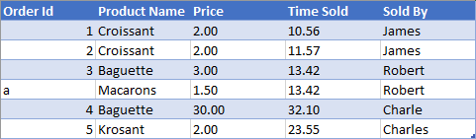
\includegraphics[width=0.9\linewidth]{thesis/Figures/DirtyDataset.png}
    \caption{Robert's data after a day of work}
    \label{fig:dirty_data_robert}
\end{figure}

Because it was the first time gathering data, some of the values might have been entered incorrectly in the Excel sheet. Nevertheless, Robert goes and makes a nice pie chart to show his boss the findings of that day. The graph in \autoref{fig:sales_pie_dirty} shows the pie chart with the revenue contribution for that day.

Immediately, his boss tells him that he does not believe this graph and walks out of the office. 
If you look closely at \autoref{fig:sales_pie_dirty}, you see that something weird has happened. Suddenly, 4 product categories are shown. "Krosant" does not even exist, so this graph cannot be correct either. Also, it could not be true that the shop got 81\% of their revenue through "Baguette", that did not feel right for Robert. Robert just experienced an example of \textbf{"Garbage in, Garbage out."} Somehow, using the data that was gathered, was not helpful at all.

\begin{figure}[h]
    \centering
    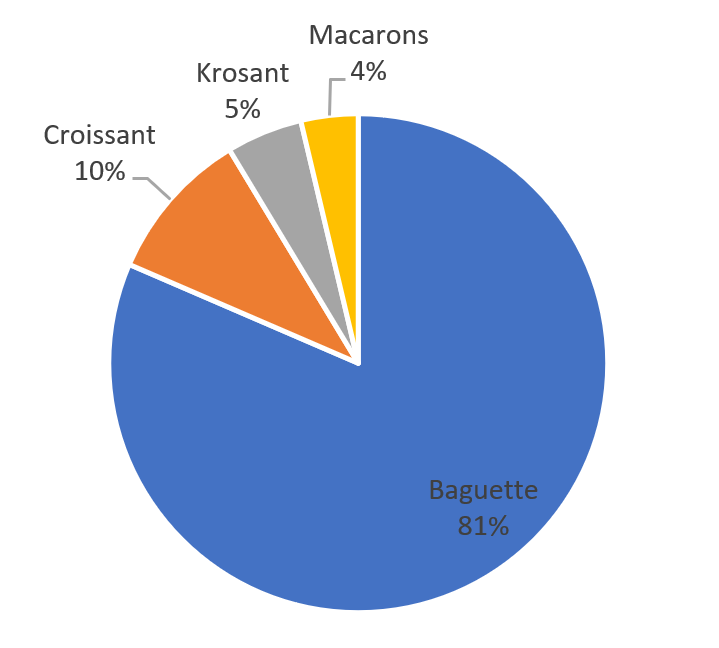
\includegraphics[width=0.5\linewidth]{thesis/Figures/Sales_Pie_Dirty.png}
    \caption{Robert's first revenue contribution chart}
    \label{fig:sales_pie_dirty}
\end{figure}

Robert quickly goes back to his sheet to see what went wrong. Taking a closer look, Robert sees that mistakes have been made. He sees that values in \autoref{fig:dirty_data_robert} cannot be true, as they do not belong to the values that can be possible. For example, "Krosant" must be "Croissant" and a "Baguette" only sells for 3.00 euros, not 30.00. The values that he altered, were \textbf{errors}. After Robert correct the data, it looked like \autoref{fig:clean_data_robert}.

\begin{figure}[h]
    \centering
    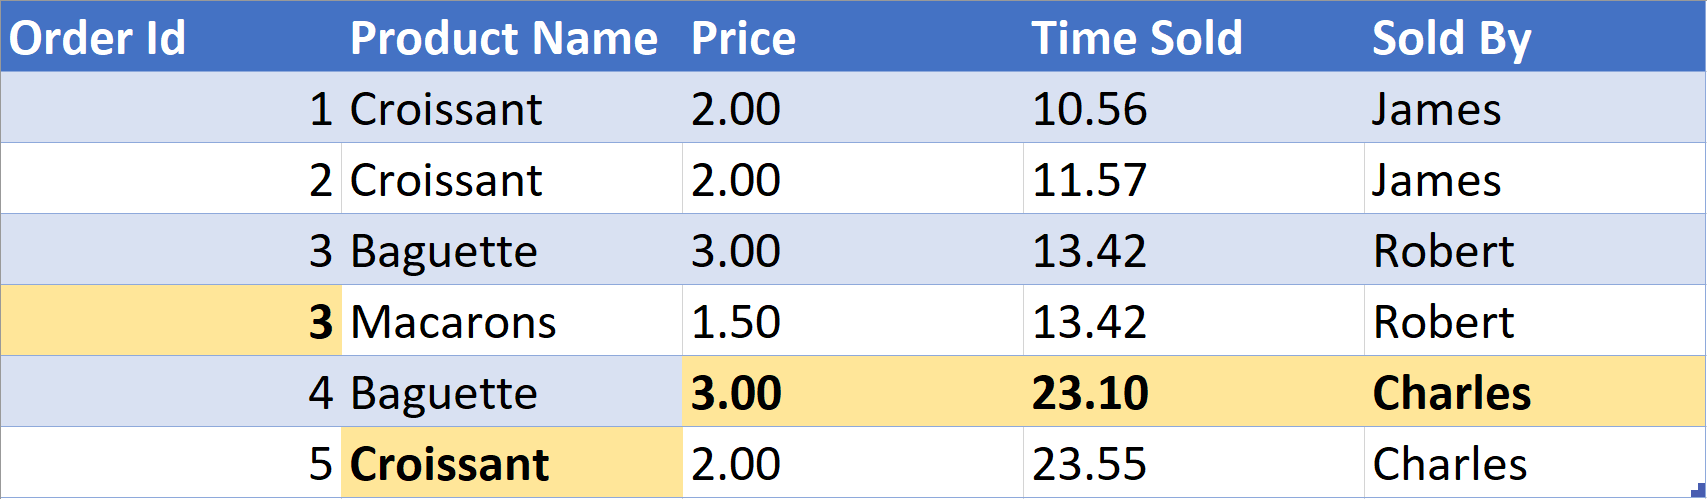
\includegraphics[width=0.9\linewidth]{thesis/Figures/CleanDataset.png}
    \caption{Robert's corrected data}
    \label{fig:clean_data_robert}
\end{figure}

Being more confident that the saved data is better now, Robert creates a new pie chart, as shown in \autoref{fig:sales_pie_clean}. Going back to his boss, he shows the new results. 
~\\The boss now trusts Robert's results and graph. The chart gives a proper idea on which of the 3 products drives revenue, giving more insights and the possibility of acting upon that insight.
And this is all the result of a single chart and well-cleaned data!

\begin{figure}[H]
    \centering
    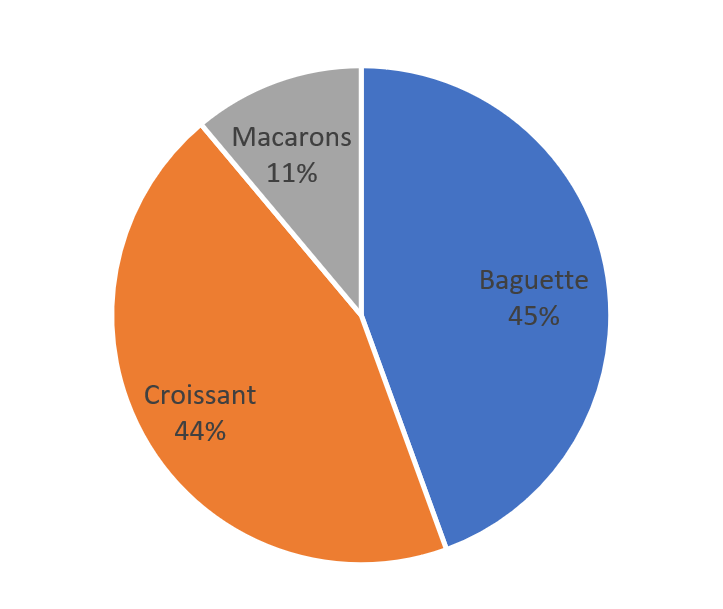
\includegraphics[width=0.5\linewidth]{thesis/Figures/Sales_Pie_Clean.png}
    \caption{Robert's corrected revenue contribution chart}
    \label{fig:sales_pie_clean}
\end{figure}

\subsection{Research topic}
The story told in the previous subsection was a story about using data. It started with collecting data. Then finding out that the collected data was not fit for generating insights. The data had to be cleaned. Data cleaning is a process that is the foundation of every individual or group that wants to do data science.

%% General part
\blockquote{Data cleaning is the process of \textbf{\textit{detecting}} and correcting (or removing) corrupt or inaccurate records from a \textbf{record set, table, or database} and refers to \textbf{identifying incomplete, incorrect, inaccurate or irrelevant parts} of the data and then replacing, modifying, or deleting the dirty or coarse data.\footnote{Definition by \cite{Wikipedia_contributors2020-ya}}}

In this thesis, the research topic will be the data cleaning process. As this process is a fairly broad concept, a more concentrated part will be focused on. Only the first step of data cleaning, the \textit{detection} of dirty data or so-called \textbf{error detection} will be the scope of this research.
As seen in the definition of data cleaning, the goal of error detection is to identify incomplete, incorrect, inaccurate or irrelevant parts of the data. 

% What are errors in relational data sources + what are relational data sources?
Moreover, the focus will be on relational data sources. These types of sources follow the relational model \cite{Codd1970-vj}. This is a structure that presents the data in tuples or rows. Each row is grouped into relations that are defined for the complete table. A relational dataset has different attributes or columns. Also, each row in that dataset will have a value for these attributes, also called a data cell. Data sources in the relational model are queryable using SQL (Structured Query Language). 

~\\The example data of \autoref{subsec:data_story} is also relational data, as shown in \autoref{fig:dirty_data_robert} and \autoref{fig:clean_data_robert}. While the data in both \autoref{fig:dirty_data_robert} and \autoref{fig:clean_data_robert} refer to the same real-world entities, events or other characteristics, there is a difference between the two. The difference between the two versions is the correction of unwanted values to the desired values. The unwanted differences are called errors.
~\\So an error in relational data is a deviation from the desired ground truth values.

% What is the problem? 
~\\The problem a user tries to solve in this domain is to identify all erroneous cells in a relational dataset. In the examples given above, manual cleaning is still possible, but with increasing size of datasets, increasing costs in cleaning arise. Luckily, there exist (semi-)automated error detection tools. These algorithms or tools try to identify erroneous cells, based on common deviations from the ground truth. These common errors could be outlying numerical values (like the "baguette" costing 30.00 euros), missing values or misspellings ("Krosant" vs "Croissant"). Questions that arise when trying to find a tool that helps to detect errors are:

\begin{itemize}
    \item Which algorithm is the best?
    \item How will it perform when I run it on my data?
    \item How to configure that tool?
    \item Why would it work and can we understand when it does not work?
\end{itemize}

These questions are the foundation of the work presented in this thesis. Now that the topic has been introduced, the motivation of the subject will be covered in the next section.